\chapter{v2 inference on real 2015 data}
\label{chap:v2real}

This chapter is the v2 counterpart of \cref{sec:v1-real-symptoms}. We
take the three v2-trained models, run them on the four months of real
2015 recordings with the same sliding-window engine
(\texttt{architectures/inference\_real\_data.py}, the same code paths
used for the v1 inference plots), and inspect the resulting per-class
confidence traces. The result is qualitative --- there is no labelled
real test set against which to compute event-level F1 --- but
unambiguous: the three v2 architecture-specific failure modes of v1
(\cref{sec:v1-real-symptoms}) are gone.

\section{v2 inference on the first month}
\label{sec:v2-real-feb}

\Cref{fig:v2-real-inference} shows the first $10\,000$ samples of
February 2015 inferred by each of the three v2 models, in the same
layout and with the same plotting conventions as
\cref{fig:v1-real-inference}.

\begin{figure}[H]
    \centering
    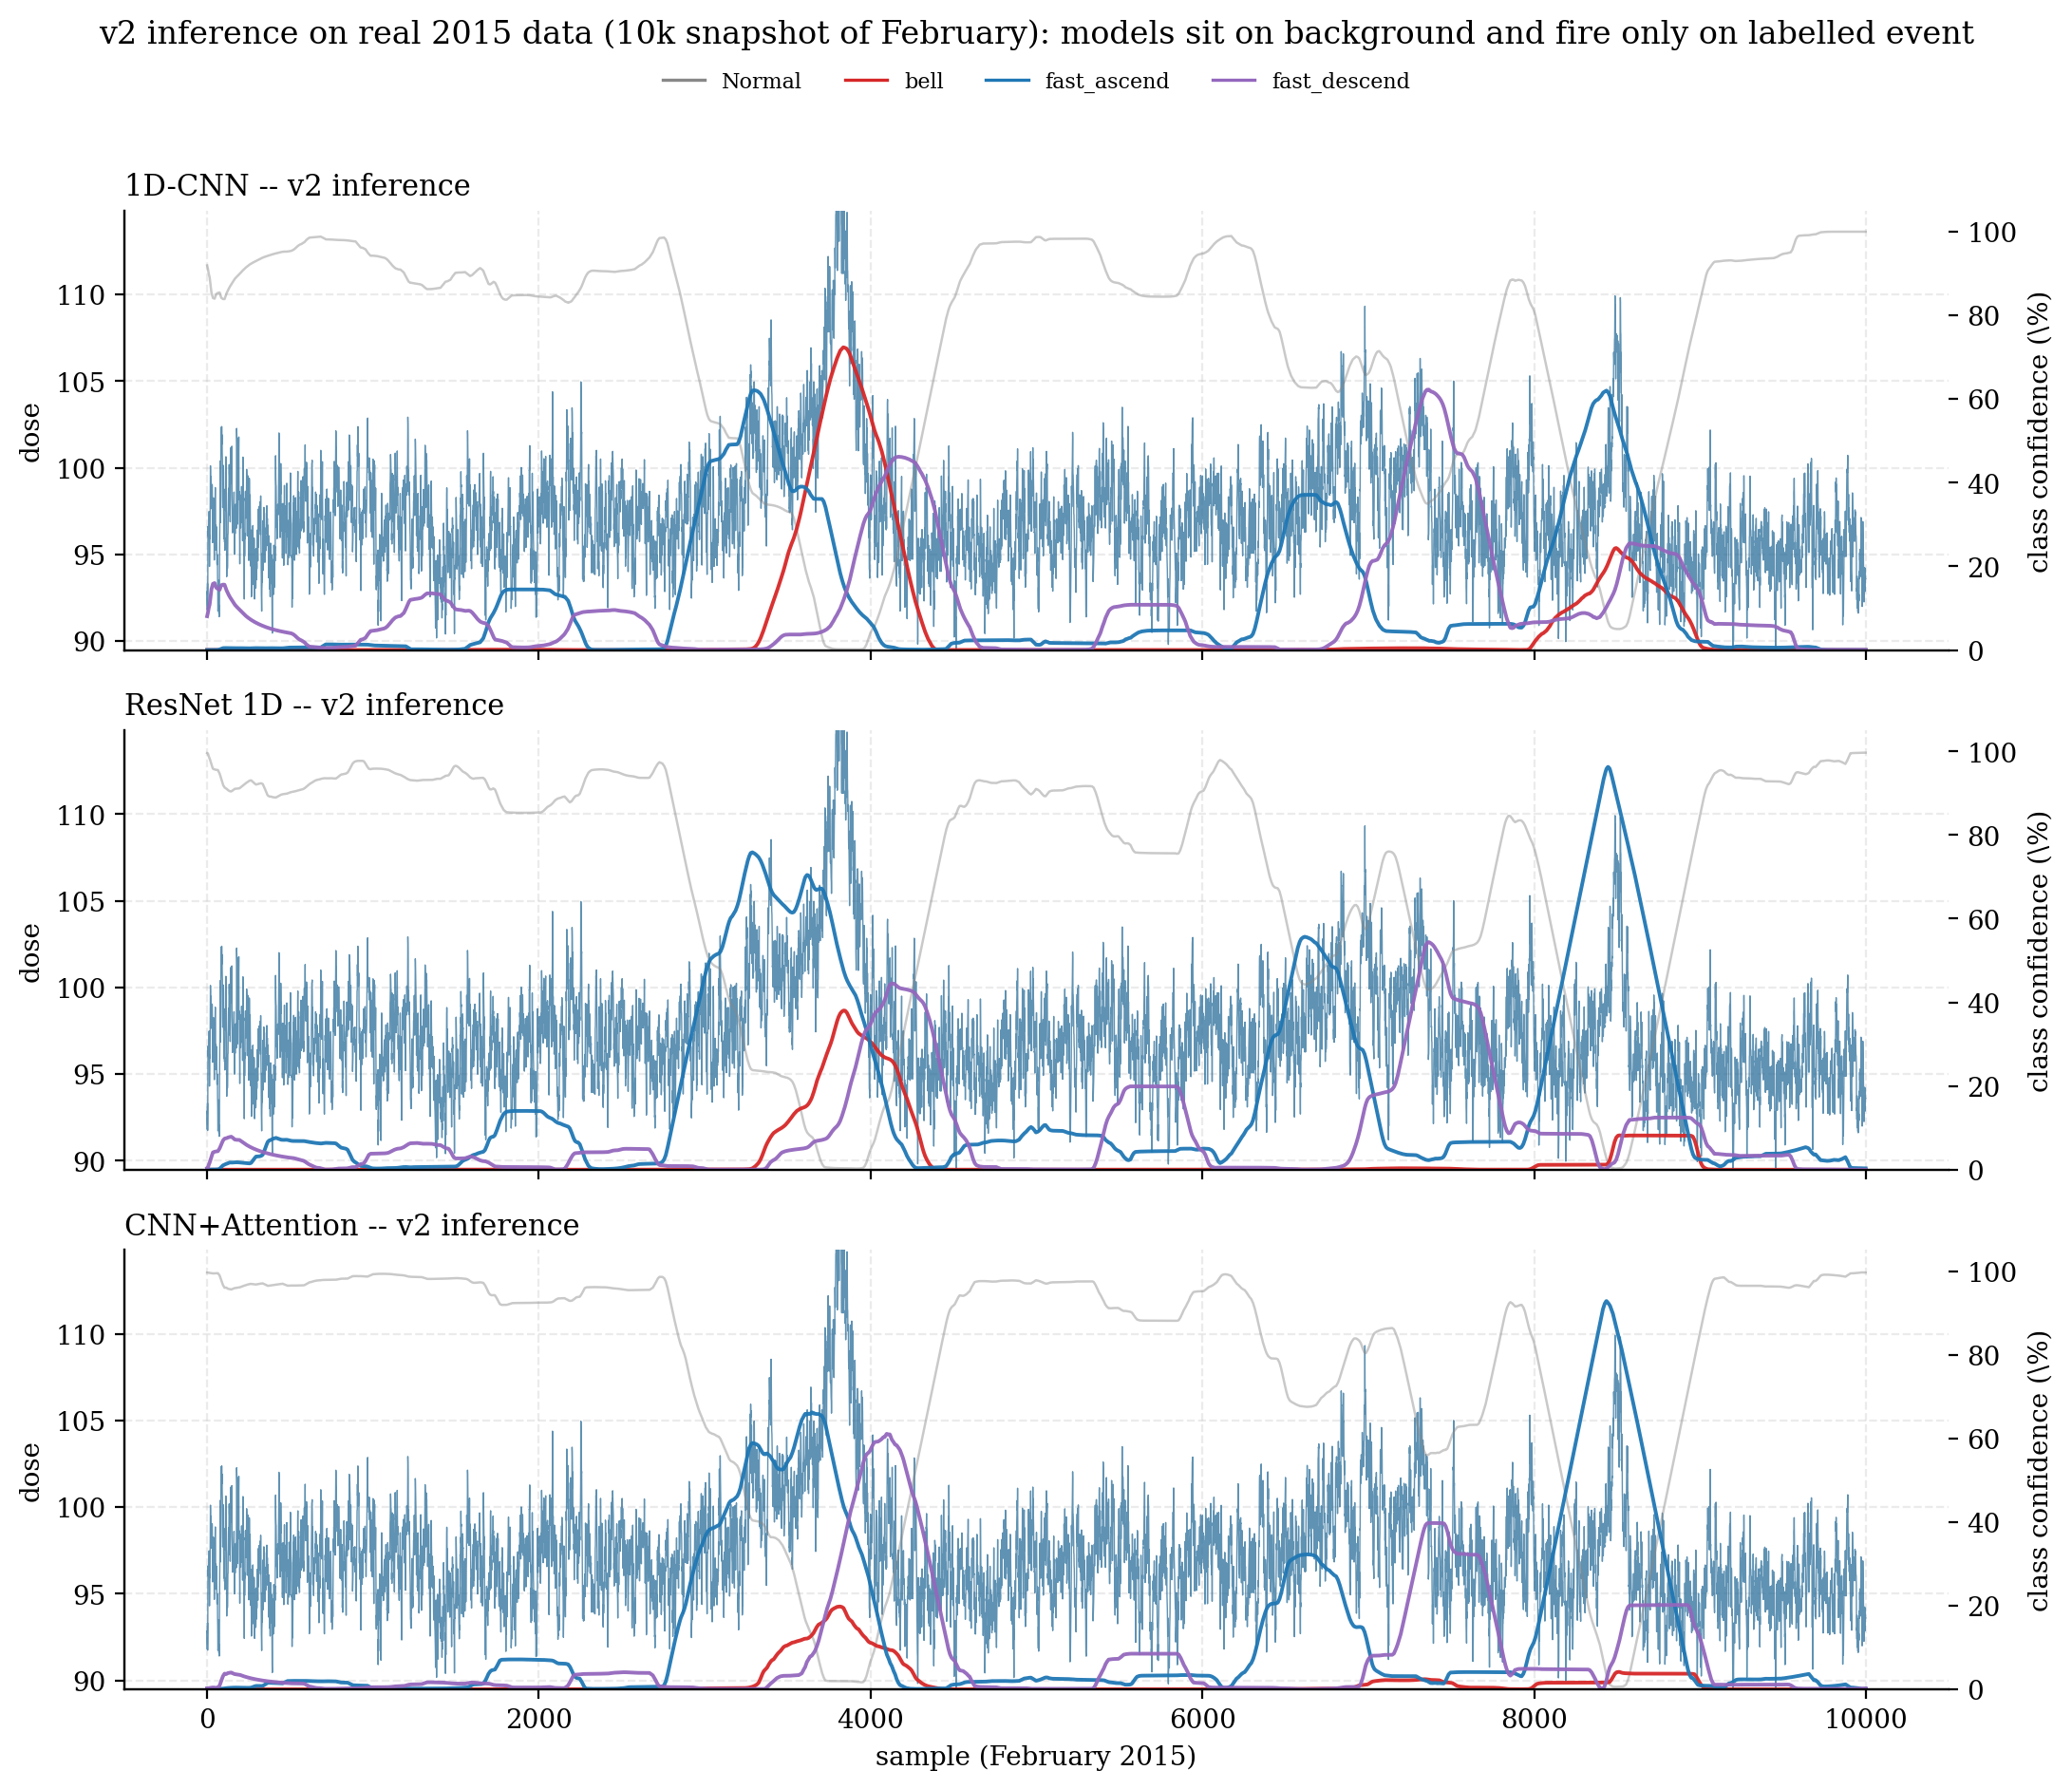
\includegraphics[width=\linewidth]{figures/v2_real_inference}
    \caption{v2 inference on the first $10\,000$ samples of February
    2015. Blue: raw gamma dose (left axis). Grey: smoothed
    \texttt{Normal Background} confidence. Coloured lines: the three
    anomaly classes (right axis, $0$--$100\%$). Compared to
    \cref{fig:v1-real-inference}, the grey background-confidence curve
    is near $100\%$ throughout the quiet regions and only drops where
    the raw signal contains a visible bump.}
    \label{fig:v2-real-inference}
\end{figure}

The three v1 failure modes of \cref{sec:v1-real-symptoms} are
individually addressed:
\begin{enumerate}[leftmargin=*, itemsep=0.2em]
    \item \textbf{1D-CNN oscillation $\rightarrow$ silent on
    background.} The background confidence is a flat ceiling near
    $100\%$ instead of a $50\%$--$70\%$ band; the model \emph{commits}
    to \texttt{Normal} on quiet regions, which is exactly the
    behaviour we want.
    \item \textbf{ResNet false-positive plateaus $\rightarrow$ gone.}
    The thousands-of-samples \texttt{bell\_sq}/\texttt{M} plateaus
    that dominated the v1 ResNet trace are no longer present; the
    model fires only at the labelled Fevereiro event around sample
    $3\,500$.
    \item \textbf{CNN+Attention collapse $\rightarrow$ no
    fixation.} The v1 model was pinned to \texttt{M} for the entire
    $10\,000$-sample window. The v2 model sits on \texttt{Normal}
    between events and produces a clear \texttt{fast\_ascend}/
    \texttt{bell} response at the labelled event. Removing the
    \texttt{M} template (the attractor of the collapse in v1) is the
    proximate cause; matching the background statistics so that the
    real signal is no longer out-of-distribution is what makes it
    stick.
\end{enumerate}

\section{Side-by-side comparison on ResNet}
\label{sec:v2-real-resnet}

The single most striking visual contrast is on the ResNet
(\cref{fig:v1-vs-v2-resnet}): v1's confident wrong answer becomes v2's
silent-then-attentive behaviour.

\begin{figure}[H]
    \centering
    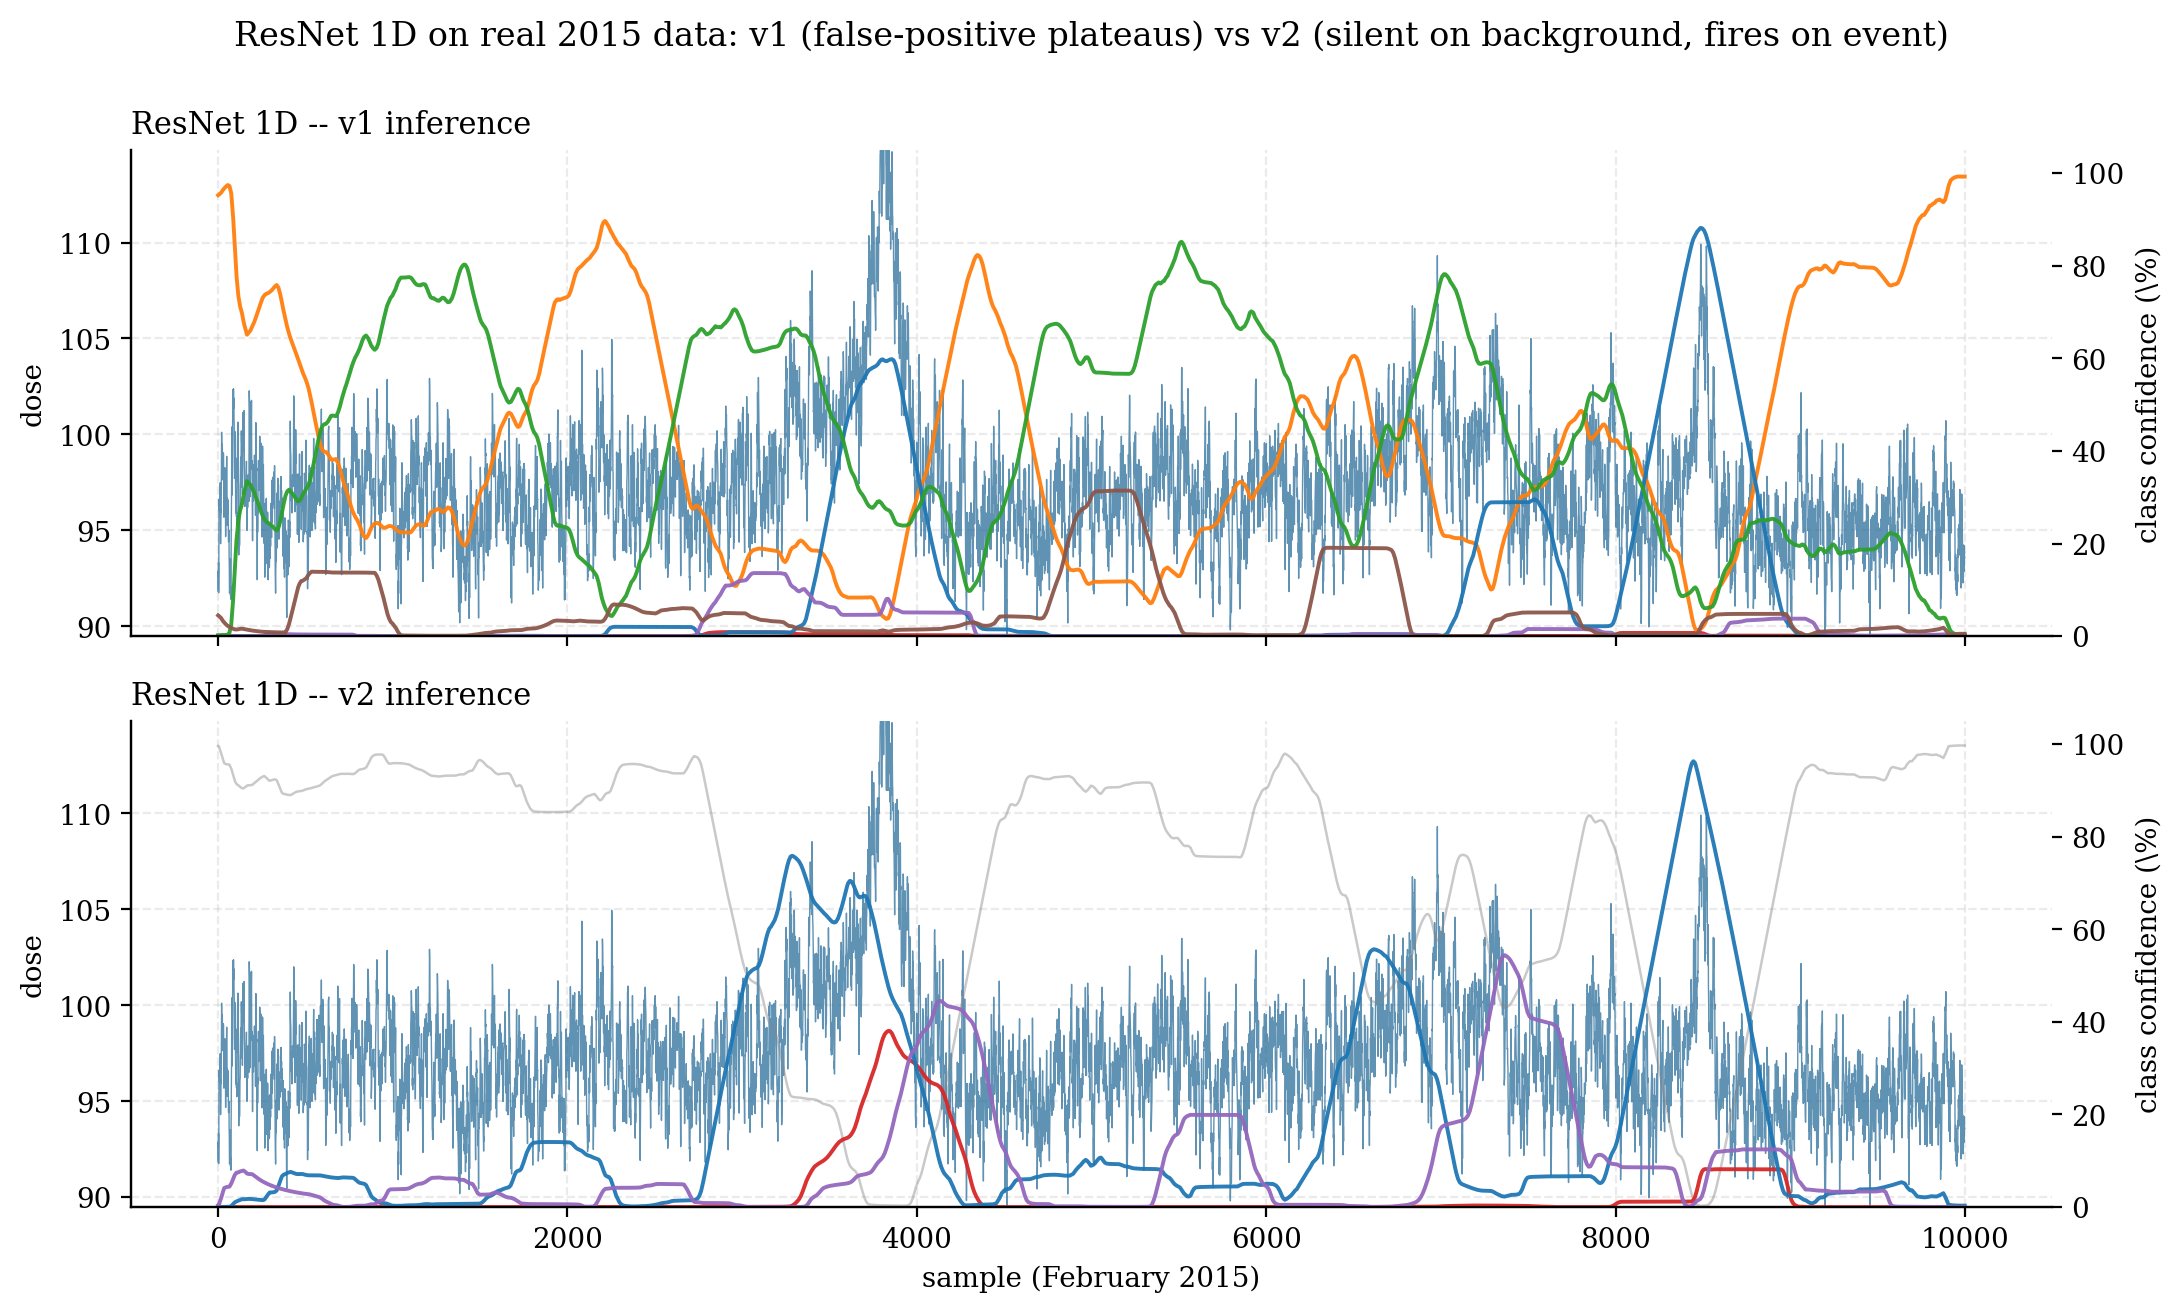
\includegraphics[width=\linewidth]{figures/v1_vs_v2_real_inference_resnet}
    \caption{ResNet 1D on the first $10\,000$ samples of February 2015.
    \textbf{Top}: v1, six classes, training on white-noise dataset ---
    sustained false-positive plateaus across the entire window.
    \textbf{Bottom}: v2, four classes, training on AR(1) dataset
    calibrated to the hand labels --- the model sits on \texttt{Normal}
    on the background and fires only at the labelled event around
    sample $3\,500$.}
    \label{fig:v1-vs-v2-resnet}
\end{figure}

\section{Caveats}
\label{sec:v2-real-caveats}

\paragraph{This is a qualitative result.} There is no labelled real
test set against which to compute event-level precision or recall.
Whether the three v2 models also detect the two additional labelled
February events (near samples $8\,500$ and $18\,800$, see
\cref{sec:reanalysis-labels}) at full confidence cannot be read off a
single $10\,000$-sample snapshot; nor can we tell whether they
correctly stay silent on the other three months.

\paragraph{Short events.} The shortest hand-labelled events (June,
$32$--$55$ samples) are well below the $W = 512$ window length but
still firmly within the range the event-coverage labelling rule
(\cref{sec:framing}, $\tau_{\text{cov}} = 0.30$) keeps in the
training distribution. The v2 synthetic-test segment of
\cref{tab:v2-event-prf} reports that events of comparable length
($26$--$45$ samples) are detected by \emph{all three} models, so the
June events are expected to be within reach of the v2 networks ---
though confirming this needs a real labelled test set, see below.

\paragraph{The next step is expert labelling.} The qualitative
improvement of v2 over v1 closes most of the synthetic--real gap that
\cref{chap:v1real} catalogued, but the remaining gap can only be
measured with proper labels. A second pass of labelling by a
radiological expert --- ideally on more than the four available
months, since seasonal effects on the background are visible in
\cref{tab:reanal-drift} --- would unlock:
\begin{itemize}[leftmargin=*, itemsep=0.2em]
    \item a real test set with which to measure event-level F1, the
    metric used for the synthetic benchmark in \cref{chap:results};
    \item refined event boundaries, which would tighten the duration
    distribution and may suggest a finer template family;
    \item detection of low-amplitude or rare-shape events that fall
    below the $\pm 2\sigma$ visibility threshold of the current
    labelling protocol.
\end{itemize}

The next chapter wraps up.
